\documentclass[conference]{IEEEtran}
\usepackage{graphicx}
\usepackage{booktabs}
\usepackage{amsmath}
\usepackage{xcolor}
\usepackage{url}
\usepackage{cite}
\providecommand{\fillin}[1]{\textcolor{red}{[#1]}}

\begin{document}

\title{OptiPIM at Reduced Scale: Reproducing ILP-Optimal\\Processing-in-Memory Mappings}

\author{\IEEEauthorblockN{Group 12: Pari Khandelwal, \fillin{Member 2}, \fillin{Member 3}, \fillin{Member 4}}
\IEEEauthorblockA{\fillin{Course name, Department, University}}}

\maketitle

\begin{abstract}
Processing-in-memory (PIM) accelerators only pay off when each operator is
mapped well onto banks, DRAM columns and time, and when its data is laid out to
match. OptiPIM (ISCA 2025) casts this mapping and layout problem as an integer
linear program (ILP) and reports large speedups over hand-written heuristics.
We reproduce its core result at reduced scale with the authors' public flow and
Gurobi: five single operators (three ResNet-50 convolutions, two BERT matrix
multiplications) on HBM-PIM and SIMDRAM, scored with the authors' analytical
model and, for three operators, their Ramulator2 simulator. OptiPIM beats the
weight-parallel heuristic by 27--34$\times$ on HBM-PIM convolutions and by
1.1--2.5$\times$ on SIMDRAM, matching the paper's trend. It loses on one
HBM-PIM matrix multiplication (0.78$\times$), which we trace to the mapping using
24 of 32 banks; the ILP objective there is two orders of magnitude below the
analytical cost; replaying both mappings in the simulator confirms the loss
(0.79$\times$). The analytical model tracks the simulator within 2.7\% on
HBM-PIM but underestimates SIMDRAM by 13--116\%. We also found that
\texttt{pim-opt} writes stride and dilation in the opposite order to the
authors' scorer. \fillin{One sentence on the extension and its result.}
\end{abstract}

\section{Introduction}
PIM architectures place compute next to (HBM-PIM~\cite{hbmpim}) or inside
(SIMDRAM~\cite{simdram}) DRAM arrays, so a deep-learning operator runs fast only
if its loops are split well across banks, columns and time steps, and its
inputs, weights and outputs are placed where the compute units can use them.
Existing PIM software uses heuristics or exhaustive or random search, and
mappers built for ASIC accelerators (e.g.\ COSA~\cite{cosa}) ignore the
data-layout costs that dominate PIM.

OptiPIM~\cite{optipim} models mapping and data layout together as one ILP,
solved to optimality by Gurobi in seconds to minutes, and reports average
speedups of 2.3$\times$ on SIMDRAM and 72.8$\times$ on HBM-PIM over the
weight-parallel heuristic. This report reproduces that comparison at the
reduced scale set for the course, checks the paper's analytical cost model
against the simulator, and \fillin{adds one extension of our own}.

Our contributions are: (1) a working build of the authors' flow on a
WSL2 laptop with Gurobi~13, including a workaround for a presolve failure;
(2) optimal mappings for five operators on both targets and a comparison with
the authors' heuristic mappings, with a reproducible scoring and plotting
pipeline; (3) a three-way comparison of ILP objective, analytical model and
simulator that exposes where they disagree; (4) \fillin{the extension}.

\section{Background: the OptiPIM Formulation}
\textbf{Targets.} HBM-PIM places a SIMD unit next to each pair of banks; its
cost is dominated by moving inputs and weights into the unit's registers.
SIMDRAM computes bit-serially inside the DRAM array, so multiplication and
addition latency dominate.

\textbf{Mapping space.} Each loop of an operator (N, K, P, Q, C, R, S for a 2D
convolution; N, K, P, Q, R for a matrix multiplication) is split into three
factors whose product is the loop bound: one across banks (level~2, parallel),
one across DRAM columns (level~1, parallel) and one over time (level~0).
OptiPIM also chooses \emph{transformation coefficients} that decide how the
indices are laid out in memory (flexible indexing), which lets the solver trade
parallelism against input reuse.

\textbf{Cost model.} The paper derives analytical expressions for computation,
output reduction and input loading (Eq.~17--19) and minimises their sum
(Eq.~20), estimating the number of unique inputs with its own counting method
(Eq.~11). The authors validate their model against a modified Ramulator2 and
report $R^2>0.99$ on both targets (Fig.~9 of~\cite{optipim}). The formulation
assumes that every loop bound factorises exactly across the three levels
(Sec.~5.1.1).

\section{Implementation and Experimental Setup}
\label{sec:setup}

\subsection{Toolchain}
We use the authors' public flow (ETHZ-DYNAMO/OptiPIM~\cite{optipimrepo},
commit 9be8f9a), forked into our group repository. It has three parts:
\texttt{pim-opt}, an MLIR pass built on LLVM (commit 39048b69) that reads one
layer in the \texttt{linalg} dialect, builds the ILP, calls Gurobi and writes
the mapping as a trace file; a Python analytical model
(\texttt{validation/analytical\_modeling}) that scores a trace with the
paper's cost model; and a modified Ramulator2~\cite{ramulator2} that replays a
trace as PIM commands and reports \texttt{memory\_system\_cycles}.

We built the flow on Ubuntu 22.04 under WSL2 on a Windows laptop (6 logical
cores and 11\,GB of RAM given to WSL, g++ 11.4.0). Building LLVM,
\texttt{pim-opt} and the simulator took about 4\,h\,15\,min. We used Gurobi
13.0.3 with a free academic licence; the paper used 11.0.3. The repository's
CMake module only searches for Gurobi 11.0 and 12.0, so we exposed the 13.0
library under the 12.0 name; no source code was changed. With Gurobi~13,
presolve wrongly reported the $3{\times}3$ convolutions C1 and C2 infeasible on
HBM-PIM at 32 banks (the same models solve at 8, 16, 17 and 20 banks), so we
solve with presolve disabled (\texttt{Presolve 0}), which gives a proven
optimum. A Dockerfile in the repository reproduces the build for members on
macOS.

\subsection{Operators and targets}
Following the reduced scope, we map five single operators rather than full
networks (Table~\ref{tab:ops}), taken from the layer files in
\texttt{nn\_models/} with the bank count set to 32. C1 is the layer the paper
analyses in its Fig.~12. Each operator is mapped onto HBM-PIM
(\texttt{--target-device-type 1}, \texttt{data/hbm\_pim.json}) and SIMDRAM
(\texttt{--target-device-type 0}, \texttt{data/dram.json}), with 16-bit values.

\begin{table}[t]
\centering
\caption{Operators used in our evaluation}
\label{tab:ops}
\footnotesize
\begin{tabular}{lll}
\toprule
ID & Source layer & Shape \\
\midrule
C1 & ResNet-50 conv12 & $3{\times}3$, 128$\to$128 ch., $28{\times}28$ out, stride 2 \\
C2 & ResNet-50 conv2  & $3{\times}3$, 64$\to$64 ch., $56{\times}56$ \\
C3 & ResNet-50 conv1  & $1{\times}1$, 64$\to$64 ch., $56{\times}56$ \\
M1 & BERT fc0         & GEMM $128{\times}768{\times}768$ \\
M2 & BERT fc1         & batched GEMM $12{\times}128{\times}64{\times}128$ \\
\bottomrule
\end{tabular}
\end{table}

\subsection{ILP configuration and solve time}
All runs use the paper's full method: flexible indexing
(\texttt{--trans-coeff-method 4}), the paper's input-counting estimate
(\texttt{--number-counting-method 0}) and the PIM cost objective
(\texttt{--obj-method 0}). One script solves all ten operator--target pairs,
stores each mapping and Gurobi log, and records solve times
(Table~\ref{tab:solve}). Every run ended with ``Optimal solution found''. Solve
times of 1.1--181\,s are in line with the paper's 1--209\,s on a consumer-grade
16-core CPU. \fillin{A rerun from a fresh clone gave identical mappings / identical objective values.}

\begin{table}[t]
\centering
\caption{Gurobi solve time per operator (seconds)}
\label{tab:solve}
\footnotesize
\begin{tabular}{lrr}
\toprule
Operator & HBM-PIM & SIMDRAM \\
\midrule
C1 & 64.2 & 44.3 \\
C2 & 181.0 & 85.0 \\
C3 & 27.5 & 5.8 \\
M1 & 2.9 & 2.4 \\
M2 & 5.8 & 1.1 \\
\bottomrule
\end{tabular}
\end{table}

\subsection{Baseline: weight-parallel heuristic}
The paper's baseline (Sec.~6.4.1) tiles the weight matrix or convolution
filters to the SIMD width and spreads the tiles over banks, columns and rows,
reloading inputs for every SIMD operation. We use the heuristic mappings the
authors ship in \texttt{baseline\_mappings/heuristic\_1} (and
\texttt{heuristic\_2} as a cross-check) for exactly our five layers at 32 banks
(ResNet50-12, -2, -1 and BERT-0, -1; problem sizes checked against our
operators). The \texttt{heuristic\_1} mapping for C1 is identical to the
paper's Fig.~12(c). \fillin{If Member 2's reimplementation exists: it reproduces these traces / differs in ...}

\subsection{Scoring}
Every mapping, OptiPIM's and the heuristic's, is scored with the same
analytical model and arch file, so speedups are unit-free. Absolute costs are
never compared across targets, because the two use different formulas and
arch files and we have not verified that both are cycles of the same clock.
Our script \texttt{group12/analysis/rerun.sh} rescores all traces and
regenerates every figure and table in this report from the committed files.

While building this pipeline we found that \texttt{pim-opt} writes the
\texttt{DilationStride} line of a trace as dilation, dilation, stride, stride
(\texttt{DataLayoutMILP.cpp}), whereas the authors' Python parser reads the
first field as stride and the third as dilation, which is also the order of
their shipped heuristic traces. Scored directly, C1 (stride 2) is treated as a
stride-1, dilation-2 convolution. Our scorer swaps the fields for
\texttt{pim-opt} traces. The fix leaves C1 on HBM-PIM unchanged (870{,}912) and
raises C1 on SIMDRAM from 24{,}995{,}102 to 26{,}701{,}846.

\section{Baseline Results Compared with the Paper}

\subsection{OptiPIM versus the heuristic}
Fig.~\ref{fig:speedup} and Table~\ref{tab:speedup} compare OptiPIM with
\texttt{heuristic\_1}. On HBM-PIM, OptiPIM is 27--34$\times$ faster on the three
convolutions and 2.8$\times$ on M2; on SIMDRAM it is 1.1--2.5$\times$ faster on
every operator (geometric mean 1.74$\times$). This matches the paper's trend:
very large wins on HBM-PIM convolutions, where the heuristic breaks input
reuse, and modest wins on SIMDRAM, where bit-serial compute dominates every
mapping (paper: 72.8$\times$ and 2.3$\times$ on average over full networks,
2.4$\times$ for BERT on HBM-PIM). Our averages are over five operators only, so
they are not directly comparable to the paper's network-level numbers.

\begin{figure}[t]
\centering
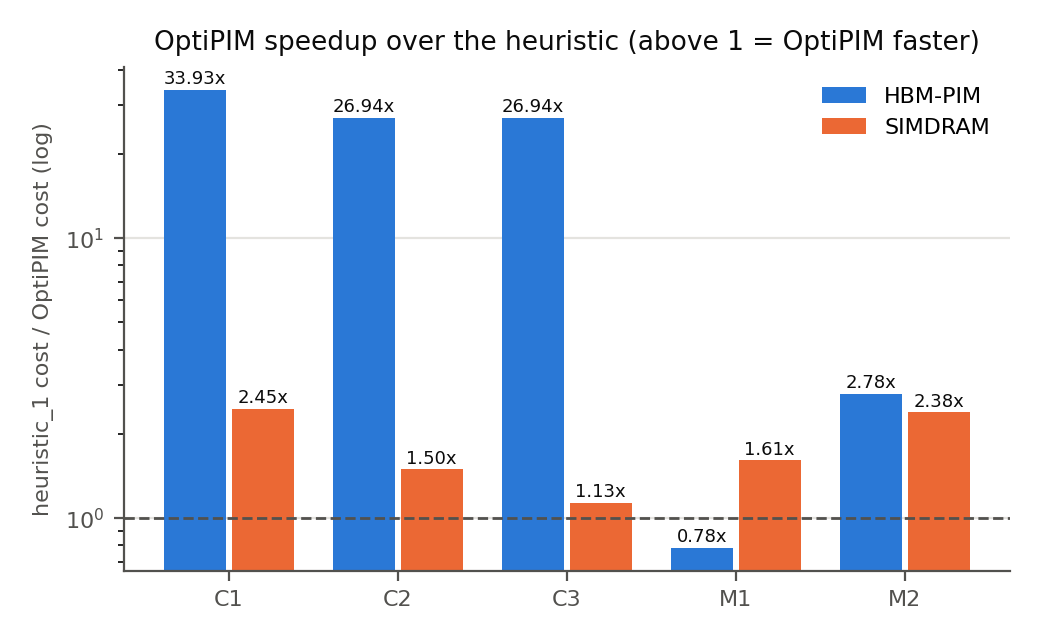
\includegraphics[width=\columnwidth]{figs/speedup.png}
\caption{OptiPIM speedup over the weight-parallel heuristic
(\texttt{heuristic\_1} cost / OptiPIM cost, analytical model, log scale).}
\label{fig:speedup}
\end{figure}

\begin{table}[t]
\centering
\caption{Analytical cost of OptiPIM and heuristic mappings, and speedup}
\label{tab:speedup}
\footnotesize
\setlength{\tabcolsep}{3pt}
\begin{tabular}{lrrrrrr}
\toprule
 & \multicolumn{3}{c}{HBM-PIM} & \multicolumn{3}{c}{SIMDRAM} \\
\cmidrule(lr){2-4}\cmidrule(lr){5-7}
Op & OptiPIM & Heur. & $\times$ & OptiPIM & Heur. & $\times$ \\
\midrule
C1 & 870{,}912 & 29{,}546{,}496 & 33.9 & 26{,}701{,}846 & 65{,}549{,}429 & 2.45 \\
C2 & 1{,}096{,}704 & 29{,}546{,}496 & 26.9 & 24{,}338{,}662 & 36{,}395{,}701 & 1.50 \\
C3 & 121{,}856 & 3{,}282{,}944 & 26.9 & 3{,}575{,}824 & 4{,}053{,}173 & 1.13 \\
M1 & 1{,}064{,}960 & 835{,}584 & \textbf{0.78} & 15{,}443{,}838 & 24{,}881{,}280 & 1.61 \\
M2 & 221{,}184 & 614{,}400 & 2.78 & 3{,}257{,}727 & 7{,}769{,}472 & 2.38 \\
\bottomrule
\end{tabular}
\end{table}

\textbf{Where OptiPIM loses: M1 on HBM-PIM.} An ILP solved to optimality cannot
lose to a heuristic if both are judged by the ILP's own cost, yet under the
analytical model OptiPIM's M1 mapping is 1.27$\times$ slower than the
heuristic's. The simulator agrees: it needs 1{,}082{,}667 cycles for the
OptiPIM mapping and 853{,}291 for the heuristic's, a ratio of 0.79$\times$
(model: 0.78$\times$). The cost breakdown pinpoints the reason: the
OptiPIM mapping uses 24 of the 32 banks, while the heuristic uses all 32. Its compute term is identical to
the heuristic's (147{,}456), and its input loading (524{,}288 vs 393{,}216) and
weight loading (393{,}216 vs 294{,}912) are both exactly $32/24=4/3$ larger,
which accounts for the whole gap. The ILP still preferred this mapping because
its HBM-PIM objective for M1 is only 9{,}888, about 108$\times$ below the
analytical cost (Section~\ref{sec:objcheck}), so it does not see the loading
costs that the extra banks would have reduced. We have not confirmed in the
ILP source which terms are missing.

\subsection{Cost breakdown}
Fig.~\ref{fig:breakdown} splits each analytical cost into the terms the model
adds up. On HBM-PIM, input loading is 85--98\% of the heuristic's cost on every
operator except M1; OptiPIM cuts it to 26--59\% of a much smaller total, at the
price of more weight loading. On SIMDRAM, bit-serial compute is 74--94\% of the
cost for both mappers. Both observations match the paper's Fig.~10(b,d):
compute dominates SIMDRAM and data loading dominates HBM-PIM.

\begin{figure}[t]
\centering
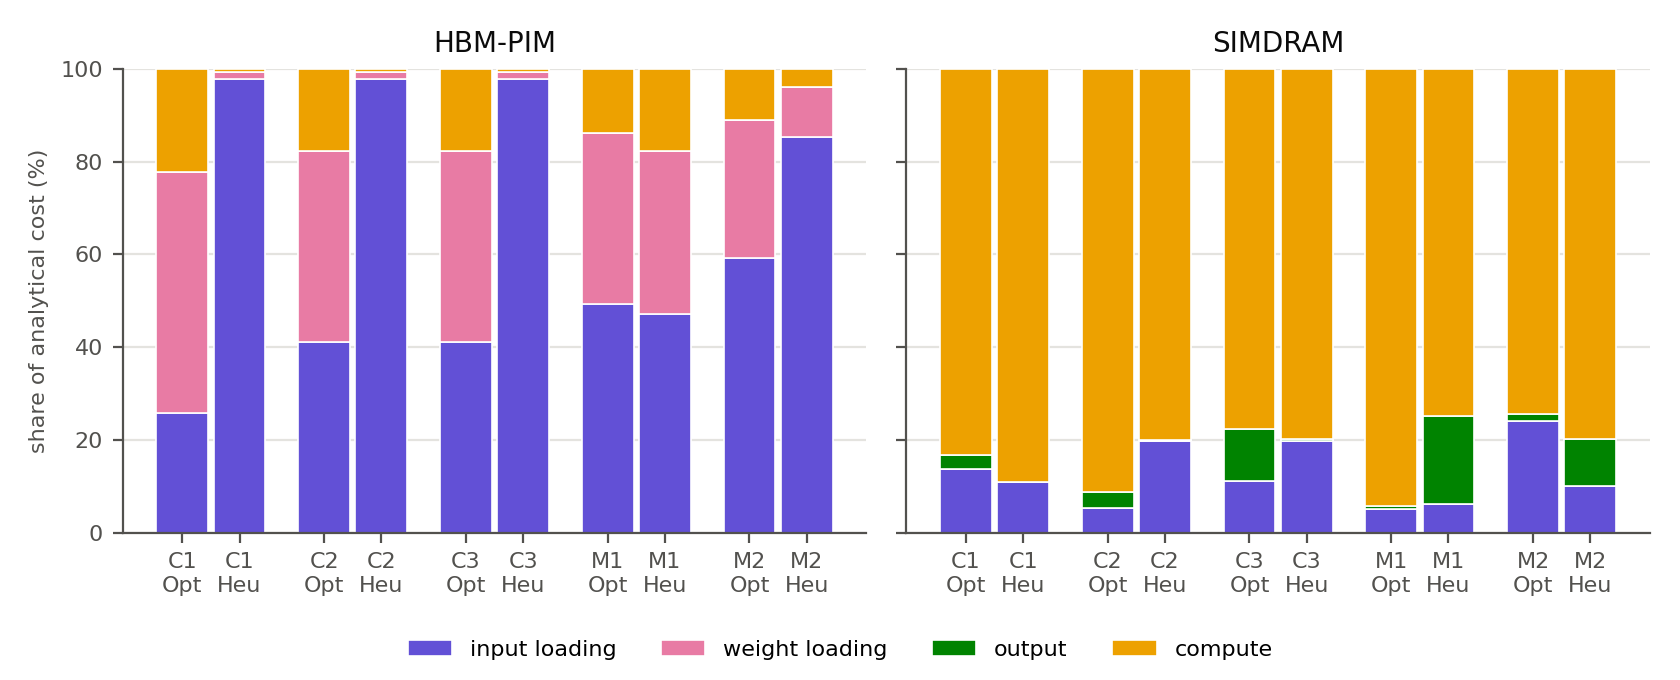
\includegraphics[width=\columnwidth]{figs/cost_breakdown.png}
\caption{Share of each cost term in the analytical model, OptiPIM (Opt) vs
\texttt{heuristic\_1} (Heu). On HBM-PIM ``compute'' is the row-activation term;
on SIMDRAM it is bit-serial multiply and add.}
\label{fig:breakdown}
\end{figure}

\subsection{Mapping case study: ResNet-50 Conv12 (C1)}
On HBM-PIM our ILP maps C1 with $Q{=}2$ and $C{=}16$ across the 32 banks,
$P{=}28$, $Q{=}2$, $C{=}8$ across columns, and $K{=}128$, $Q{=}7$, $R{=}S{=}3$
in time. The heuristic instead puts $K$ across banks and reloads the input for
every filter, so its input loading is 28{,}901{,}376 against OptiPIM's
225{,}792, which accounts for almost all of the 34$\times$ gap. The paper's
Fig.~12 reports about 100$\times$ for this layer with a different OptiPIM
mapping that uses 16 banks. We rebuilt the paper's Fig.~12(b) mapping as a trace
(its $R$ and $S$ coefficients are not shown, so we set them as in our
mapping) and scored it: 3{,}161{,}088, i.e.\ 9.3$\times$ better than the
heuristic and 3.6$\times$ worse than our 32-bank mapping. Its output-reduction
term (6{,}272) equals the value printed in the paper, but its input loading
(903{,}168) does not (18{,}432), so the costs in the paper's Fig.~12 appear to be
in different units from the Python model; we therefore compare ratios only.

\subsection{Analytical model versus simulator}
\label{sec:simcheck}
We replayed the OptiPIM and the heuristic mapping of all five operators on
both targets (20 mappings) in Ramulator2 (Fig.~\ref{fig:sim},
Table~\ref{tab:sim}). On HBM-PIM the model is within 2.7\% of the simulator for
all ten mappings replayed, consistent with the paper's Fig.~9. On SIMDRAM the
model underestimates the simulator for every mapping, by 13\% to 116\%, and by
different amounts for the two mappers (e.g.\ 41\% for OptiPIM but 13\% for the
heuristic on M1, but 97\% against 33\% on C1), so the error is not a constant
factor. The largest gaps are the two $3{\times}3$ convolutions: the simulator reports the same 52{,}540{,}980
cycles for C1 and C2, matching the identical ILP objective of their mappings
(23{,}273{,}702), while the model scores C1 10\% higher than C2. The authors' own
validation data (\texttt{exp\_results/fig9}) agrees within a few percent on
SIMDRAM, so the gap is specific to our mappings or our simulator build; we did
not find its cause.

The simulator also lets us check the speedups of Table~\ref{tab:speedup}. On
HBM-PIM they agree: 33.0$\times$ (C1), 26.4$\times$ (C2), 26.4$\times$ (C3),
0.79$\times$ (M1) and 2.75$\times$ (M2) against 33.9$\times$, 26.9$\times$,
26.9$\times$, 0.78$\times$ and 2.78$\times$ from the model. On SIMDRAM OptiPIM is
still faster for all five operators, but by 1.66$\times$ (C1), 1.13$\times$ (C2),
1.34$\times$ (C3), 1.29$\times$ (M1) and 1.88$\times$ (M2) instead of
2.45$\times$, 1.50$\times$, 1.13$\times$, 1.61$\times$ and 2.39$\times$ (geometric
mean 1.44$\times$ instead of 1.74$\times$), so the model gets the direction right
but not the size of the gain.

\begin{figure*}[t]
\centering
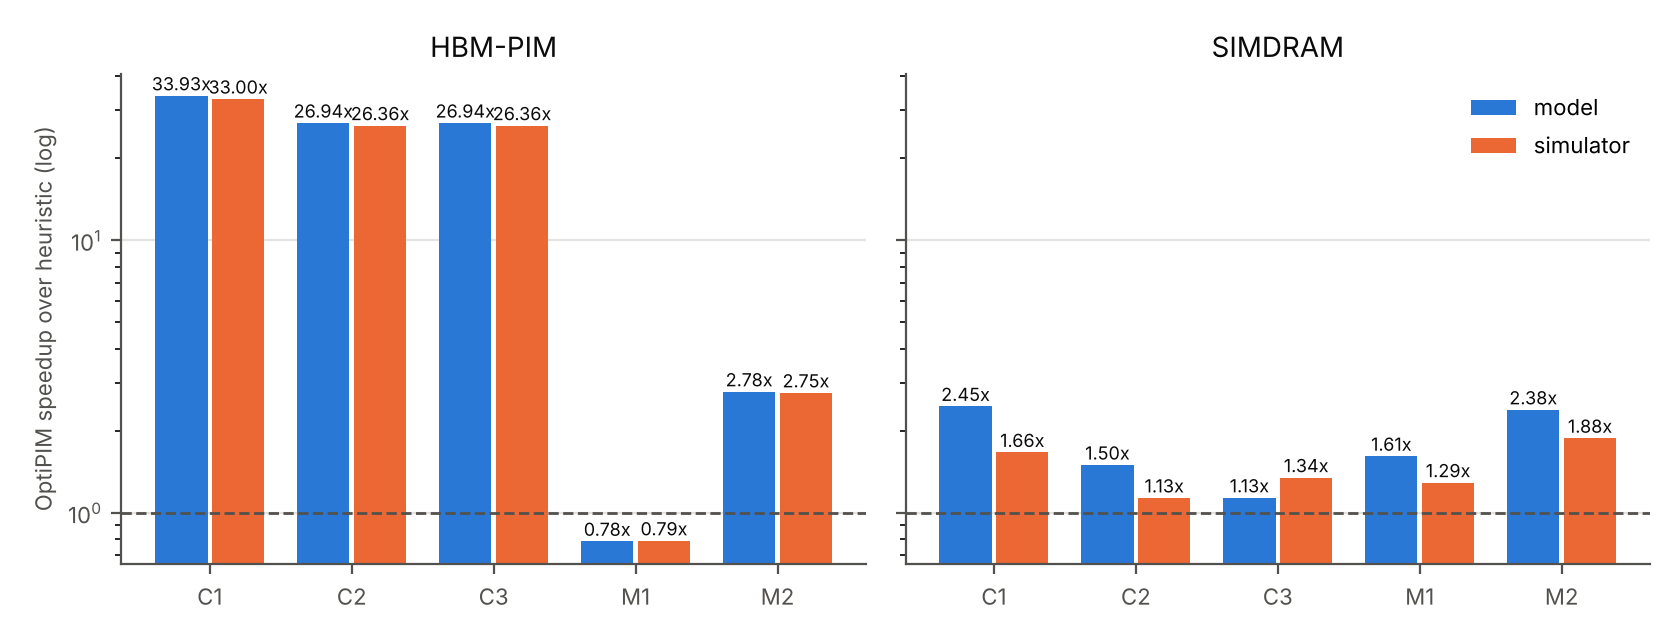
\includegraphics[width=0.85\textwidth]{figs/speedup_model_vs_sim.png}
\caption{OptiPIM speedup over the heuristic according to the analytical model
and to the Ramulator2 simulator (log scale).}
\label{fig:simspeedup}
\end{figure*}

\begin{figure}[t]
\centering
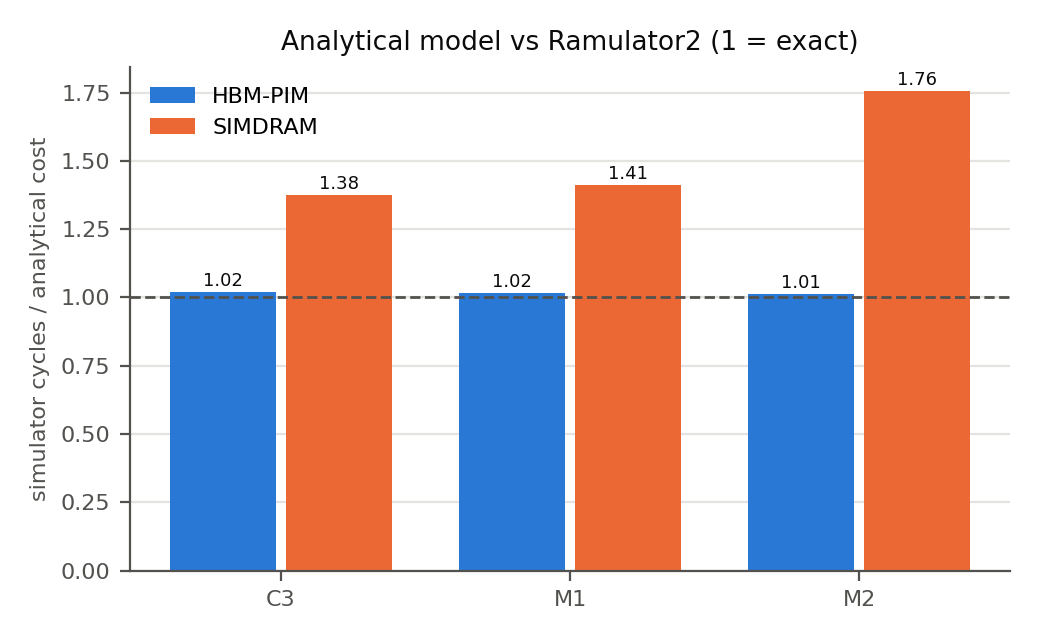
\includegraphics[width=\columnwidth]{figs/analytical_vs_sim.png}
\caption{Simulator cycles divided by analytical cost for OptiPIM mappings
(1 = exact agreement). The heuristic mappings are in Table~\ref{tab:sim}.}
\label{fig:sim}
\end{figure}

\begin{table}[t]
\centering
\caption{Analytical model versus Ramulator2 (cycles)}
\label{tab:sim}
\footnotesize
\begin{tabular}{llrrr}
\toprule
Op, mapper & Target & Model & Simulator & Diff. \\
\midrule
C1 OptiPIM & HBM-PIM & 870{,}912 & 894{,}779 & $+2.7\%$ \\
C2 OptiPIM & HBM-PIM & 1{,}096{,}704 & 1{,}120{,}256 & $+2.1\%$ \\
C1 heuristic & HBM-PIM & 29{,}546{,}496 & 29{,}529{,}983 & $-0.1\%$ \\
C2 heuristic & HBM-PIM & 29{,}546{,}496 & 29{,}529{,}983 & $-0.1\%$ \\
C3 OptiPIM & HBM-PIM & 121{,}856 & 124{,}464 & $+2.1\%$ \\
C3 heuristic & HBM-PIM & 3{,}282{,}944 & 3{,}281{,}117 & $-0.1\%$ \\
M1 OptiPIM & HBM-PIM & 1{,}064{,}960 & 1{,}082{,}667 & $+1.7\%$ \\
M1 heuristic & HBM-PIM & 835{,}584 & 853{,}291 & $+2.1\%$ \\
M2 OptiPIM & HBM-PIM & 221{,}184 & 224{,}061 & $+1.3\%$ \\
M2 heuristic & HBM-PIM & 614{,}400 & 616{,}797 & $+0.4\%$ \\
C1 OptiPIM & SIMDRAM & 26{,}701{,}846 & 52{,}540{,}980 & $+96.8\%$ \\
C2 OptiPIM & SIMDRAM & 24{,}338{,}662 & 52{,}540{,}980 & $+115.9\%$ \\
C1 heuristic & SIMDRAM & 65{,}549{,}429 & 87{,}405{,}433 & $+33.3\%$ \\
C2 heuristic & SIMDRAM & 36{,}395{,}701 & 59{,}496{,}616 & $+63.5\%$ \\
C3 OptiPIM & SIMDRAM & 3{,}575{,}824 & 4{,}919{,}252 & $+37.6\%$ \\
C3 heuristic & SIMDRAM & 4{,}053{,}173 & 6{,}612{,}996 & $+63.2\%$ \\
M1 OptiPIM & SIMDRAM & 15{,}443{,}838 & 21{,}804{,}288 & $+41.2\%$ \\
M1 heuristic & SIMDRAM & 24{,}881{,}280 & 28{,}097{,}818 & $+12.9\%$ \\
M2 OptiPIM & SIMDRAM & 3{,}257{,}727 & 5{,}725{,}248 & $+75.8\%$ \\
M2 heuristic & SIMDRAM & 7{,}769{,}472 & 10{,}739{,}994 & $+38.2\%$ \\
\bottomrule
\end{tabular}
\end{table}

\subsection{Solver objective versus analytical model}
\label{sec:objcheck}
Table~\ref{tab:obj} compares the ILP objective with the analytical cost of the
same mapping. On SIMDRAM they agree within 5--32\%. On HBM-PIM the model's cost
is 2.4--3.0$\times$ the objective for the convolutions and 73--108$\times$ for
the matrix multiplications. \texttt{pim-opt} also prints its own ``Real Cost''
after solving (176{,}544 for M1 on HBM-PIM), which matches neither. The
objective is therefore not a cycle count, and on HBM-PIM matrix
multiplications it ranks mappings differently from the model that the
simulator confirms, which is how the M1 loss arises.

\begin{table}[t]
\centering
\caption{ILP objective and analytical cost of the OptiPIM mappings}
\label{tab:obj}
\footnotesize
\setlength{\tabcolsep}{4pt}
\begin{tabular}{lrrrr}
\toprule
 & \multicolumn{2}{c}{HBM-PIM} & \multicolumn{2}{c}{SIMDRAM} \\
\cmidrule(lr){2-3}\cmidrule(lr){4-5}
Op & ILP & Model & ILP & Model \\
\midrule
C1 & 360{,}149 & 870{,}912 & 23{,}273{,}702 & 26{,}701{,}846 \\
C2 & 364{,}316 & 1{,}096{,}704 & 23{,}273{,}702 & 24{,}338{,}662 \\
C3 & 45{,}906 & 121{,}856 & 3{,}174{,}416 & 3{,}575{,}824 \\
M1 & 9{,}888 & 1{,}064{,}960 & 14{,}632{,}830 & 15{,}443{,}838 \\
M2 & 3{,}040 & 221{,}184 & 2{,}471{,}295 & 3{,}257{,}727 \\
\bottomrule
\end{tabular}
\end{table}

\subsection{Summary of differences from the paper}
\begin{itemize}
\item HBM-PIM M1: OptiPIM 0.78$\times$ the heuristic because it uses 24 of 32
banks; the ILP objective does not reflect the loading costs (above).
\item SIMDRAM model-vs-simulator gap of 13--116\%, not seen in the paper, and
different for the two mappers, so the model also misjudges the size of the
SIMDRAM speedups.
\item Smaller C1 gain (34$\times$ vs about 100$\times$); the paper's Fig.~12
costs are in different units, and its mapping uses 16 banks.
\item Gurobi 13.0.3 instead of 11.0.3, with presolve disabled; with several
optimal solutions a different version may return a different mapping.
\item Five single operators instead of whole networks, so we cannot reproduce
the paper's per-network averages.
\end{itemize}

\section{Our Contribution: \fillin{Extension Title}}
\label{sec:ext}
\fillin{Member 4 to complete with results. Planned design below (idea A).}

\textbf{Limitation in the paper's words.} OptiPIM ``assume[s] a perfect
factorization of the original loop bound'' (Sec.~5.1.1): every loop factor is
chosen from the exact divisors of the bound. A prime or awkward bound, such as
197 tokens in ViT attention or 50{,}257 in the GPT-2 output layer, cannot be
spread across banks or SIMDRAM columns, so lanes sit idle.

\textbf{Hypothesis.} Zero-padding an awkward bound to a nearby 7-smooth size
(e.g.\ 197$\to$200) gives the ILP many more legal factorisations; the better
mapping can outweigh the extra work on padded elements.

\textbf{What we built.} \texttt{pad\_search.py} rewrites a layer with padded
bounds (each dimension $\le$25\% larger, total MACs $\le$30\% larger), runs the
unchanged \texttt{pim-opt} on each candidate, rescores every result with the
analytical model, and keeps the cheapest; the unpadded layer is always a
candidate, so the search never loses to the baseline.

\textbf{Evaluation.} Best padded mapping vs OptiPIM on the exact shape vs the
heuristic, on \fillin{N} awkward shapes and both targets.

\textbf{Results.} \fillin{Figure and table from run\_padding\_eval.sh, rescored with score\_traces.py.}
A cheap compute-only prescreen predicts gains mainly on SIMDRAM (about
1.6$\times$ for ViT attention, 1.1--1.2$\times$ for ViT QKV and GPT-2) and none on
HBM-PIM; \fillin{state whether the ILP results confirm this}.

\textbf{Discussion.} \fillin{When padding helps, when it does not, and its cost (extra memory, host zero-fill).}

\section{Limitations of Our Setup}
\label{sec:limits}
\begin{itemize}
\item \textbf{No real hardware.} All cycle counts come from the analytical
model and the authors' Ramulator2-based simulator.
\item \textbf{Few simulator points.} We simulated 20 mappings (two per operator
and target), against the paper's 12{,}000 random mappings, and one run each, so
we cannot report an $R^2$ comparable to the paper's.
\item \textbf{Unexplained gaps.} The SIMDRAM model-vs-simulator gap and the
ILP-objective-vs-model gap on HBM-PIM are measured but not explained.
\item \textbf{Different solver version and machine.} Gurobi 13.0.3 with
presolve disabled, on a laptop rather than the paper's setup; absolute solve
times are not comparable.
\item \textbf{Five operators, one configuration.} 32 banks and 16-bit values
only.
\item \textbf{Heuristic baseline.} We use the authors' shipped heuristic
mappings rather than the original HBM-PIM software.
\end{itemize}

\section{What We Left Out}
\begin{table}[h]
\centering
\caption{Parts of the paper left out and what we used instead}
\label{tab:leftout}
\footnotesize
\begin{tabular}{p{0.42\columnwidth}p{0.48\columnwidth}}
\toprule
Paper & Our setup \\
\midrule
Real-hardware measurements & Analytical model and Ramulator2 simulator \\
PIM-DL genetic-search baseline & Weight-parallel heuristic only \\
Full networks (AlexNet, ResNet, VGG, UNet, BERT, Llama) & Five single operators from ResNet-50 and BERT \\
Memory scalability study & 32 banks only \\
PyTorch $\to$ Torch-MLIR front end & The authors' shipped \texttt{.linalg.mlir} layer files \\
COSA-style ASIC mapping baseline & Not run \\
\bottomrule
\end{tabular}
\end{table}

\section{Conclusion}
With the authors' flow and Gurobi~13 we reproduced OptiPIM's main trend at
reduced scale: large wins over the weight-parallel heuristic on HBM-PIM
convolutions and modest wins on SIMDRAM. The reproduction also exposed three
weak points that the paper's averages hide: a matrix multiplication where the
ILP picks a mapping slower than the heuristic because its objective diverges
from the validated cost model, a SIMDRAM model-vs-simulator gap, and a
stride/dilation ordering mismatch between \texttt{pim-opt} and its scorer.
\fillin{One sentence on the extension.}

\section*{Member Contributions}
\textbf{Pari Khandelwal} (Member 1) built the toolchain (LLVM, \texttt{pim-opt},
Ramulator2) and the Gurobi setup on WSL2, diagnosed the Gurobi~13 presolve
failure, solved all operators on both targets, wrote the scoring, simulator and
plotting scripts, found the stride/dilation mismatch, wrote the Dockerfile and
build instructions, and wrote the setup, results and limitations sections.
\textbf{\fillin{Member 2}}: \fillin{heuristic baseline}.
\textbf{\fillin{Member 3}}: \fillin{evaluation and simulator correlation}.
\textbf{\fillin{Member 4}}: \fillin{extension}.

\section*{Code}
All source code, mappings, results and build instructions:
\url{https://github.com/parikhwal291/OptiPIM-grp12}. \texttt{group12/README.md}
explains the build; \texttt{bash group12/analysis/rerun.sh . . group12/results/plots}
regenerates every figure and table in this report.

\begin{thebibliography}{9}
\bibitem{optipim} J.~Liu \emph{et~al.}, ``OptiPIM: Optimizing processing-in-memory acceleration using integer linear programming,'' in \emph{Proc. ISCA}, 2025.
\bibitem{optipimrepo} ETHZ-DYNAMO, ``OptiPIM,'' GitHub repository. [Online]. Available: \url{https://github.com/ETHZ-DYNAMO/OptiPIM}
\bibitem{hbmpim} S.~Lee \emph{et~al.}, ``Hardware architecture and software stack for PIM based on commercial DRAM technology,'' in \emph{Proc. ISCA}, 2021.
\bibitem{simdram} N.~Hajinazar \emph{et~al.}, ``SIMDRAM: A framework for bit-serial SIMD processing using DRAM,'' in \emph{Proc. ASPLOS}, 2021.
\bibitem{cosa} Q.~Huang \emph{et~al.}, ``CoSA: Scheduling by constrained optimization for spatial accelerators,'' in \emph{Proc. ISCA}, 2021.
\bibitem{pimdl} C.~Li \emph{et~al.}, ``PIM-DL: Expanding the applicability of commodity DRAM-PIMs for deep learning via algorithm-system co-optimization,'' in \emph{Proc. ASPLOS}, 2024.
\bibitem{ramulator2} H.~Luo \emph{et~al.}, ``Ramulator 2.0: A modern, modular, and extensible DRAM simulator,'' \emph{IEEE Comput. Archit. Lett.}, 2023.
\bibitem{gurobi} Gurobi Optimization, LLC, ``Gurobi Optimizer Reference Manual,'' 2024.
\end{thebibliography}

\end{document}
